%==============================
\section{Online Human Interaction and Request Fulfillment}
\label{ch05:sec:ch05_human}


\subsection{Request-consistent Embedded Graph Instantiation}
\label{ch05:subsec:requests}
Built on the latency-bounded communication, this section
presents the request-instantiation layer of {MoRoCo}. Given the
wheel backbone and an incoming request, it constructs a
request-consistent embedded graph together with the resized backbone and the detach schedule. It then introduces the
procedure to compute this transition, followed by the
request-specific graph constructions and detach--rejoin executions.


% =========================================================
\subsubsection{Problem of Request-consistent Graph Instantiation}

Within {MoRoCo}, each request~$\xi$ in
Table~\ref{ch05:tab:requests} is realized through a family of candidate
embedded target graphs that encode the desired robot roles and
communication topology, denoted by~$\widehat{\mathcal{G}}_k^{\xi}$.
Given the current embedded wheel backbone graph
$\mathcal{G}_k^{\texttt{w}}$, the request-instantiation problem seeks: a resized wheel backbone $\mathcal{G}_k^{\texttt{w'}}$,
a selected target graph
$\mathcal{G}_k^{\xi}\in\widehat{\mathcal{G}}_k^{\xi}$,
and the corresponding detach events
$\widehat{\pi}_k^{\xi}\triangleq\{\pi_r^{\xi}\}$ that realize the
required topology transition. The performance measure is given by:
% ====================
\begin{equation}\label{ch05:eq:match_objective}
  \underset{\mathcal{G}_k^{\texttt{w'}},\,\mathcal{G}_k^{\xi},\,
  \widehat{\pi}_k^{\xi},\,\Pi_k^{\xi}}{\textbf{min}}
\Big(
T_k^{\texttt{trs}}(\mathcal{G}_k^{\texttt{w}},\,
\mathcal{G}_k^{\texttt{w'}})
+ w_{\texttt{n}} \,
\underset{r \in \mathcal{N}_k^{\xi}}{\textbf{max}}
\left\{ T_r^{\texttt{nav}}(\pi_r^{\xi},\Pi_k^{\xi}) \right\} \Big),
\end{equation}
% ====================
where
$T_k^{\texttt{trs}}(\mathcal{G}_k^{\texttt{w}},\,
\mathcal{G}_k^{\texttt{w'}})$ is the transition time induced by
resizing the wheel backbone;
$T_r^{\texttt{nav}}(\pi_r^{\xi},\Pi_k^{\xi})$ is the navigation time for robot~$r$
to execute its detach event and reach the role specified by the
assignment $\Pi_k^{\xi}$;
$\mathcal{N}_k^{\xi}$ is the set of robots that switch from
$\mathcal{G}_k^{\texttt{w}}$ to~$\mathcal{G}_k^{\xi}$; and
$w_{\texttt{n}}>0$ trades off the backbone-transition time and the
request-realization time.

% =========================================================
\begin{problem}\label{ch05:prob:graph_matching}
Given the current wheel backbone graph~$\mathcal{G}_k^{\texttt{w}}$
and the candidate target graphs~$\widehat{\mathcal{G}}_k^{\xi}$ for
request~$\xi$, define a graph instantiation procedure:
% ====================
\begin{equation}\label{ch05:eq:single_graphmatch}
  \mathcal{G}_k^{\texttt{w'}},\,\mathcal{G}_k^{\xi},\,
  \widehat{\pi}_k^{\xi},\,\Pi_k^{\xi}
  = \texttt{GraphMatch}\!\left(\mathcal{G}_k^{\texttt{w}},\,
  \widehat{\mathcal{G}}_k^{\xi},\,\xi\right),
\end{equation}
% ====================
which realizes a request-consistent topology transition by minimizing
the objective in~\eqref{ch05:eq:match_objective}.
\end{problem}
% =========================================================


%==============================
\begin{algorithm}[t!]
\caption{Request-consistent graph instantiation for a given
request $\texttt{GraphMatch}(\cdot)$}
\label{ch05:alg:graphmatch}
\LinesNumbered
\SetKwInOut{Input}{Input}
\SetKwInOut{Output}{Output}

\Input{$\mathcal{G}_k^{\texttt{w}}$, request $\xi$, candidate set
$\widehat{\mathcal{G}}_k^{\xi}$, weight $w_{\texttt{n}}$}
\Output{$\mathcal{G}_k^{\xi}$, $\mathcal{G}_k^{\texttt{w'}}$,
$\widehat{\pi}_r^{\xi}$, $\Pi_k^{\xi}$}

Extract $\mathcal{C}^+_k$ from $\mathcal{G}_k^{\texttt{w}}$\;
\While{candidates in $\widehat{\mathcal{G}}_k^{\xi}$ remain}{
  Select candidate graph $\mathcal{G}_k^{\xi}$ given
  $\mathcal{C}^+_k, \mathbf{p}_0^{\xi}$ by
  \eqref{ch05:eq:graphmatch_next_candidate}\;
  Extract $\mathcal{N}_k^{\xi}, \mathbf{p}_0^{\xi}$ from
  $\mathcal{G}_k^{\xi}$\;
  $\mathcal{G}_k^{\texttt{w'}} \leftarrow
  \mathcal{G}_k^{\texttt{w}}[\mathcal{N}_k\setminus
  \mathcal{N}_k^{\xi}]$\;

  $(T_{\texttt{trs}},\,\widehat{\pi}_r^{\xi})
  \leftarrow
  \texttt{MultiDetach}(\mathcal{G}_k^{\texttt{w}},\,
  \mathcal{N}_k^{\xi})$ by \eqref{ch05:eq:graphmatch_trs}\;

  $\Pi_k^{\xi} \leftarrow
  \texttt{LBAP}(\mathcal{N}_k^{\xi},\,\mathbf{p}_0^{\xi},\,
  \widehat{\pi}_r^{\xi})$ by \eqref{ch05:eq:role_assignment}\;

  Update best $\widehat{\mathcal{G}}_k^{\xi}$ by
  \eqref{ch05:eq:match_objective}\;
}
\Return $\mathcal{G}_k^{\xi}$, $\mathcal{G}_k^{\texttt{w'}}$,
$\widehat{\pi}_r^{\xi}$, $\Pi_k^{\xi}$ with the best candidate\;
\end{algorithm}
%==============================


%==============================
\begin{figure*}[t!]
  \centering
  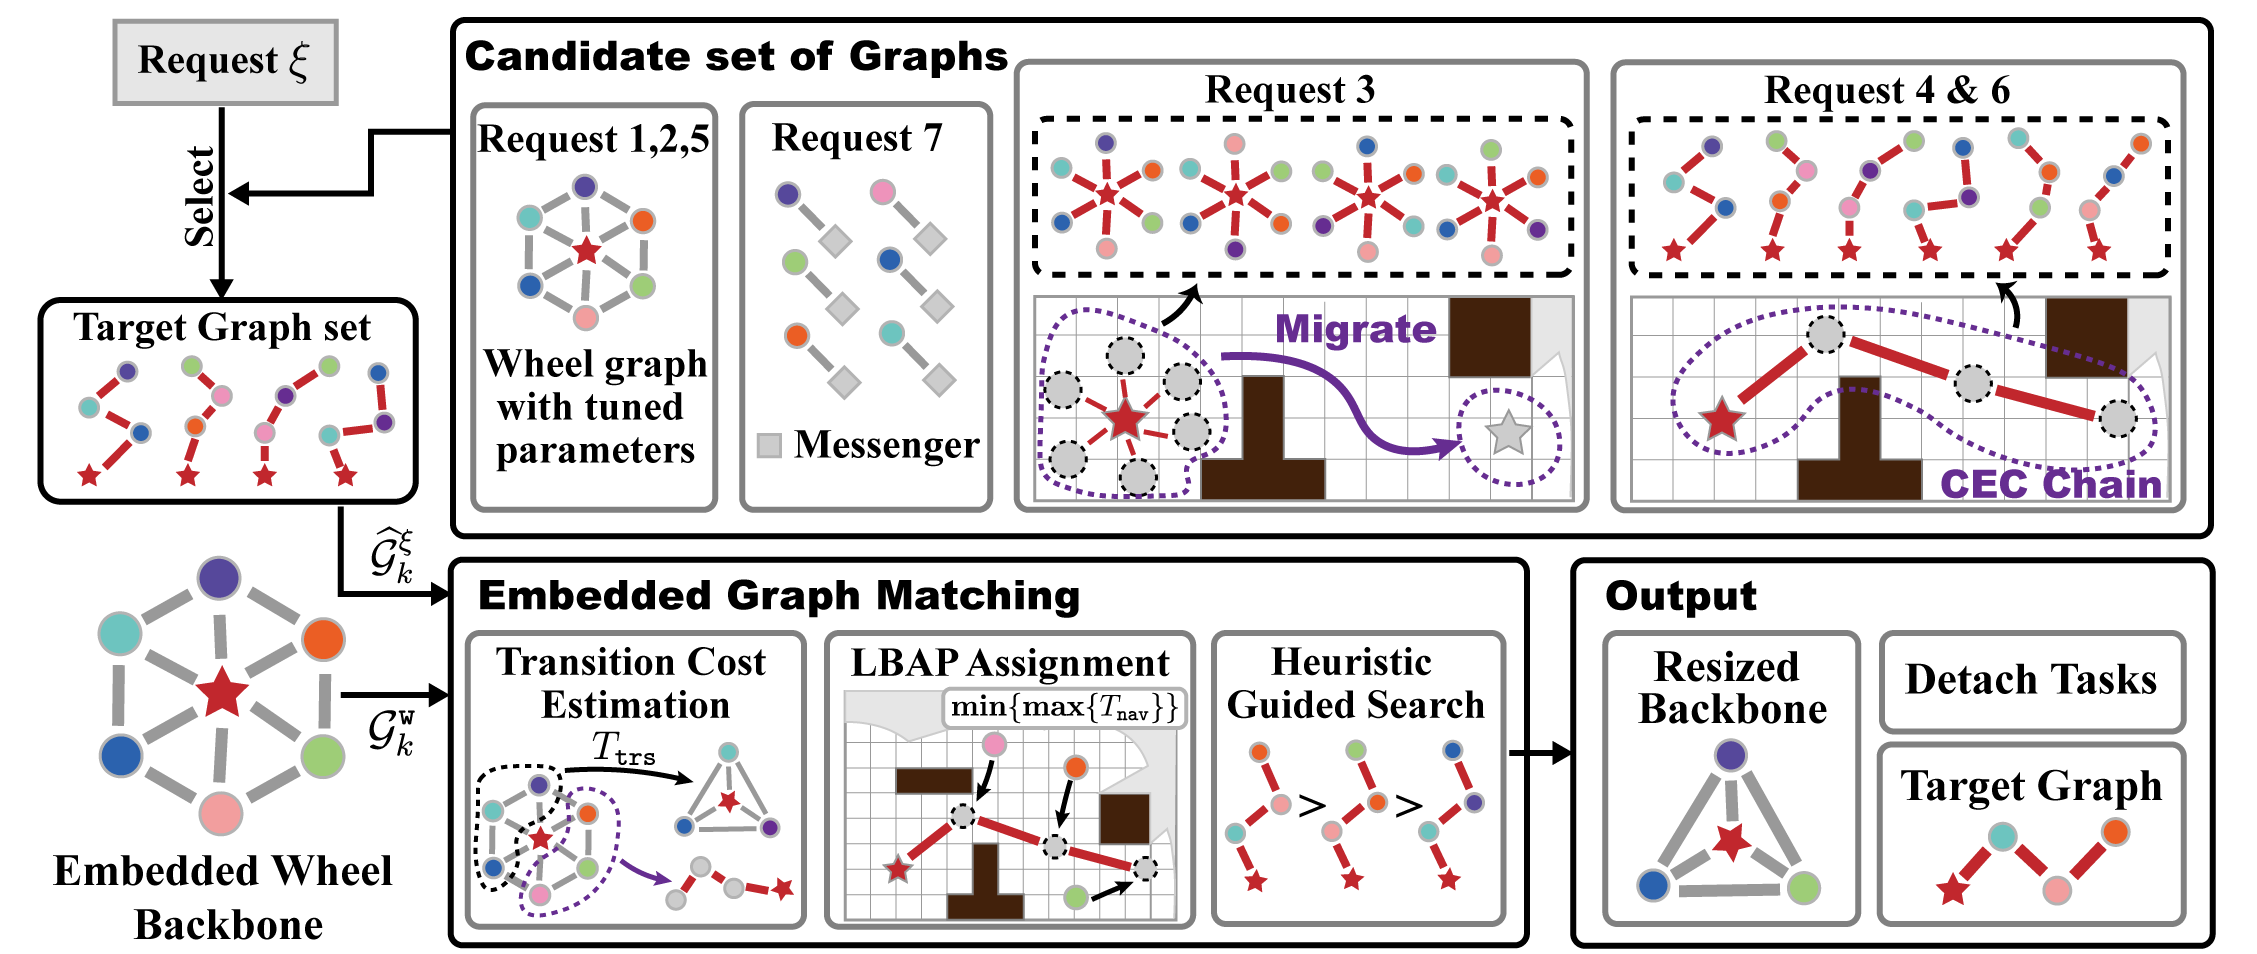
\includegraphics[width=0.93\linewidth]{figures/ch05/Graph_matching.png}
  \vspace{-2mm}
  \caption{Illustration of the request-consistent procedure of graph
    instantiation. Given a request~$\xi$
    and its associated set of candidate graphs~$\widehat{\mathcal{G}}_k^{\xi}$ (\textbf{Top}),
    \texttt{GraphMatch} selects a target graph among the set,
    and realizes it given the current wheel backbone
  $\mathcal{G}_k^{\texttt{w}}$, yielding a resized backbone~$\mathcal{G}_k^{\texttt{w'}}$, the
  instantiated target graph~$(\mathcal{G}_k^{\xi}, \Pi_k^{\xi})$, and the detach events~$\widehat{\pi}_r^{\xi}$ (\textbf{Bottom}).}
  \label{ch05:fig:graph-matching}
\end{figure*}
%==============================


% =========================================================
% =========================================================
\subsubsection{Optimization Procedure}
As illustrated in
Fig.~\ref{ch05:fig:graph-matching}, given a request-induced candidate set
$\widehat{\mathcal{G}}_k^{\xi}$, it first computes a feasible
transition schedule to resize the wheel backbone, then assigns
detached robots to target roles through an unbalanced linear
bottleneck assignment, and finally traverses the candidate set to
return the solution that minimizes
\eqref{ch05:eq:match_objective}.

The first step evaluates the transition time required to resize the
current wheel backbone into a feasible smaller wheel. For a candidate
$\mathcal{G}_k^{\xi}\in\widehat{\mathcal{G}}_k^{\xi}$, let
$\mathcal{N}_k^{\xi}$ denote the robots allocated to
$\mathcal{G}_k^{\xi}$. Removing $\mathcal{N}_k^{\xi}$ from the wheel
backbone $\mathcal{G}_k^{\texttt{w}}$ yields the resized wheel
$\mathcal{G}_k^{\texttt{w'}}$. Conditioned on the return robot that
conveys the request, the detachment routine in
Sec.~\ref{ch05:sec:detach-join} is invoked to produce a feasible timed
schedule and its transition time:
\begin{equation}
\Big(T_{\texttt{trs}}(\mathcal{G}_k^{\texttt{w}},\,
\mathcal{G}_k^{\texttt{w'}}),\,
\widehat{\pi}_r^{\xi}\Big)
\triangleq
\texttt{MultiDetach}\!\left(\mathcal{G}_k^{\texttt{w}},\,
\mathcal{N}_k^{\xi}\right),
\label{ch05:eq:graphmatch_trs}
\end{equation}
where each $\widehat{\pi}_r^{\xi}\triangleq (r,\,t_r,\,p_r)$
specifies the detach time and detach location of robot~$r$. The
transition completion time $T_{\texttt{trs}}$ is the earliest time
when $\mathcal{G}_k^{\texttt{w'}}$ is fully formed and its embeddings
are updated by~\eqref{ch05:eq:embed-update}.

In the second step, the detached robots are assigned to the role
locations of the selected target graph $\mathcal{G}_k^{\xi}$. Let
$\mathbf{p}_0^{\xi}\triangleq
\{p^\xi_{r}\}_{r\in \mathcal{N}_k^{\xi}}$ be the initial role
locations in $\mathcal{G}_k^{\xi}$. An assignment
$\Pi_k^{\xi}:\mathcal{N}_k^{\xi}\to\mathbf{p}_0^{\xi}$ induces the
bottleneck arrival time
$\textbf{max}_{r\in\mathcal{N}_k^{\xi}}
\{t_r+T_\texttt{nav}^{r}(p_r,\Pi_k^{\xi}(r))\}$,
where $T_\texttt{nav}^{r}(p_r,\Pi_k^{\xi}(r))$ is the navigation time
from the detach location to the assigned role. Selecting
$\Pi_k^{\xi}$ to minimize this term yields an unbalanced linear
bottleneck assignment problem (LBAP)~\cite{burkard2012assignment}:
\begin{equation}\label{ch05:eq:role_assignment}
  \Pi_k^{\xi} \leftarrow \texttt{LBAP}\!\left(\mathcal{N}_k^{\xi},\,
  \mathbf{p}_0^{\xi},\, \widehat{\pi}_r^{\xi}\right),
\end{equation}
which can be solved efficiently by off-the-shelf tools such as
OR-Tools~\cite{gor}, and returns a concrete role assignment
and the navigation plans for all detached robots.

The final step traverses the candidate set
$\widehat{\mathcal{G}}_k^{\xi}$ using a best-first heuristic. After
evaluating the current candidate $\mathcal{G}_{k,q}^{\xi}$, the next
candidate is selected by ranking the remaining graphs via the
surrogate score below, derived from \eqref{ch05:eq:match_objective}:
%==========================================
\begin{equation}\label{ch05:eq:graphmatch_next_candidate}
\mathcal{G}_{k,q+1}^{\xi}
=
\underset{\mathcal{G}\in\widehat{\mathcal{G}}_k^{\xi}\setminus
\{\mathcal{G}_{k,q}^{\xi}\}}{\textbf{argmin}}
\big(
\widetilde{T}_k^{\texttt{trs}}(\mathcal{G},\mathcal{C}_k^{+})
+
w_{\texttt{n}}\,
\widetilde{T}_k^{\texttt{nav}}(\mathbf{p}_0^{\xi},\mathcal{C}_k^{+})
\big),
\end{equation}
%==========================================
where $\mathcal{C}_k^{+}$ is the set of subsequent meeting events to
be executed as implied by the local plans $\{\Gamma_i\}$. Here
$\widetilde{T}_k^{\texttt{trs}}(\mathcal{G},\mathcal{C}_k^{+})$ and
$\widetilde{T}_k^{\texttt{nav}}(\mathbf{p}_0^{\xi},\mathcal{C}_k^{+})$
are fast predictors of the transition completion time and bottleneck
arrival time, respectively, conditioned on the confirmed meeting
events $\mathcal{C}_k^{+}$. This heuristic prioritizes candidates
that are likely to admit early feasible detachment and short
worst-case travel, while avoiding repeated evaluation of exact
durations during the search. The overall realization procedure is
summarized in Alg.~\ref{ch05:alg:graphmatch}. Its role within MoRoCo is to
return an executable request-consistent transition for a given
candidate family, as formalized by the following lemma and its proof
provided in the Appendix.

\begin{lemma}\label{ch05:thm:graphmatch-exec-short}
For any request $\xi$ for team $\mathcal{T}_k$, suppose there exists at
least one candidate $\mathcal{G}_k^{\xi}\in\widehat{\mathcal{G}}_k^{\xi}$
such that \eqref{ch05:eq:graphmatch_trs} returns a detach schedule for the
associated robot set $\mathcal{N}_k^{\xi}$. Then
Alg.~\ref{ch05:alg:graphmatch} terminates in finite time and returns
$(\mathcal{G}_k^{\texttt{w'}},\,\mathcal{G}_k^{\xi},\,
\widehat{\pi}_k^{\xi}, \Pi_k^{\xi})$, such that the
resulting transition is executable under the detach mechanism and the
objective in~\eqref{ch05:eq:match_objective} is minimized over all
candidates in $\widehat{\mathcal{G}}_k^{\xi}$.
\end{lemma}

% =========================================================
\subsubsection{Request-Specific Execution Modes}
\label{ch05:subsubsec:request}
Requests are executed either by updating the
embeddings of the wheel backbone or by instantiating a
request-specific embedded subgraph through the detach--execute--rejoin
mechanism. When a request requires a topology transition,
Alg.~\ref{ch05:alg:graphmatch} is invoked to instantiate a feasible target
subgraph and return role assignments together with timed detach events
for the involved robots, while the remaining robots preserve the wheel
backbone to maintain latency-bounded intermittent communication.

(I) \textbf{Intra-team communication with bounded latency.}
For intra-team exploration requests $\xi^k_1$, $\xi^k_2$, and
$\xi^k_5$, the joint-wheel backbone $\mathcal{G}^{\texttt{w}}_k$ is
retained and no subgraph instantiation is required. The base request
$\xi^k_1$ is satisfied directly by the backbone, which enforces the
latency-bounded information flow. Requests $\xi^k_2$ and $\xi^k_5$ are
realized by modifying the embeddings in~\eqref{ch05:eq:embed-update} under
the same topology. Specifically, $\xi^k_2$ excludes frontiers inside
the prohibited region~$\mathcal{P}^-$ and prioritizes other frontiers
toward $\mathcal{P}^+$ via the embedded weights:
\begin{equation}\label{ch05:eq:frontier_weight}
J(f) \triangleq \sum_{p\in \mathcal{P}^+}\Vert x(f)-p\Vert, \quad
\forall f\in \mathcal{F}_k,
\end{equation}
such that larger $J(f)$ is deprioritized. Request $\xi^k_5$ appends an
immediate return opportunity for timely delivery of $D_i$, updating the
relevant time-stamps in the embeddings without changing
$\mathcal{G}^{\texttt{w}}_k$ for the remaining period.

(II) \textbf{Inter-team exchange with bounded latency.}
For the inter-team request $\xi^{k_1k_2}_7$, neighboring teams
$\mathcal{T}_{k_1}$ and $\mathcal{T}_{k_2}$ periodically exchange
compressed mission data under the inter-team bound $T_{\texttt{c}}$.
This request is realized as a singleton messenger subgraph, where a
messenger robot detaches from its backbone, reaches an external meeting
event $\mathbf{c}_{\texttt{e}}=(p_{\texttt{e}},t_{\texttt{e}})$,
exchanges data, and rejoins. Feasibility with respect to the intra-team
meeting sequence is enforced by selecting a messenger robot from the
most recent intra-team meeting pair and scheduling the external event
according to:
\begin{equation}\label{ch05:eq:interteam_req}
\begin{aligned}
  & t_{ij}^{+} + T_{\ell}^{\texttt{nav}} \ge t_{\texttt{e}},\;
  \forall \ell\in\{i,j\}, \\
  & p_{\texttt{e}}^{+}=\mathop{\mathbf{argmin}}\limits_{p \in
    \boldsymbol{\tau}_{k_1k_2}}
    \left\{\mathop{\mathbf{max}}\limits_{\ell=k_1,k_2}
    \Big\{T_{\texttt{m}_\ell}^{\texttt{nav}}
    (p_{\texttt{h}_\ell},\,p)\Big\}\right\},
\end{aligned}
\end{equation}
where $\mathbf{c}_{ij}^{+}=(p_{ij}^{+},t_{ij}^{+})$ is the next
intra-team meeting event and $\boldsymbol{\tau}_{k_1k_2}$ is the
shortest path between operator locations $p_{\texttt{h}_{k_1}}$ and
$p_{\texttt{h}_{k_2}}$. The inter-team meeting time is advanced by
$t_{\texttt{e}}^{+}\triangleq t_{\texttt{e}}+T_{\texttt{c}}^{k_1k_2}$,
after which the messenger rejoins the backbone.

(III) \textbf{Operator relocation and group migration.}
Request $\xi^k_3$ relocates the operator $\texttt{h}_k$ to a target
position $p_{\texttt{h}_k}^+$ while preserving latency feasibility. If
$p_{\texttt{h}_k}^+$ satisfies:
%==============================
\begin{equation}\label{ch05:eq:base-location}
T_i^{\texttt{nav}}(p^+_{\texttt{h}_k},\, p^{\ell_i}_i)\leq
T_i^{\texttt{nav}}(p_{\texttt{h}_k},\, p^{\ell_i}_i),\,
\forall i\in \mathcal{N}_k,\, \ell_i\leq L_i;
\end{equation}
%==============================
then the embeddings are updated in place and the backbone topology
remains unchanged. Otherwise, the relocation is realized as a
connectivity-preserving migration. In this case, \texttt{GraphMatch}
instantiates an embedded star subgraph centered at $\texttt{h}_k$ and
assigns robots to relative placements that maintain connectivity during
motion, after which the wheel backbone is restored for continued
exploration.

(IV) \textbf{Consistent link via a communication-ensured chain.}
Requests $\xi^k_4$ and $\xi^k_6$ require a reliable and consistent
chain between the operator $\texttt{h}_k$ and a designated robot at
$p_i^\star$, as required in Def.~\ref{ch05:def:chain}. Accordingly, MoRoCo
realizes these requests through a communication-ensured chain (CEC) by
selecting anchor points along the shortest path from $p_{\texttt{h}_k}$
to $p_i^\star$ such that the hop-by-hop link quality satisfies:
\begin{equation}\label{ch05:eq:cec}
\mathbf{p}_k^{\xi}\triangleq p_0p_1\cdots p_C,\quad
\texttt{Qual}(p_c,p_{c+1},\mathcal{M}_{\texttt{h}_k})
\ge \underline{\delta}^{\texttt{c}};
\end{equation}
allocating robots to these anchor points yields an embedded chain
subgraph that enforces multi-hop connectivity based on estimated
communication quality. Unassigned robots continue exploration within
the reduced wheel backbone.


% ========================================
\subsection{Online Coordination for Multiple Simultaneous Requests}
\label{ch05:subsec:online}
This section presents the online coordination layer of
{MoRoCo} for handling multiple simultaneous requests.
Starting from the single-request instantiation mechanism introduced
above, MoRoCo handles multiple requests online by checking request
admissibility on the current wheel backbone and sequentially
instantiating feasible request subgraphs.

%==============================
\begin{figure}[t!]
    \centering
    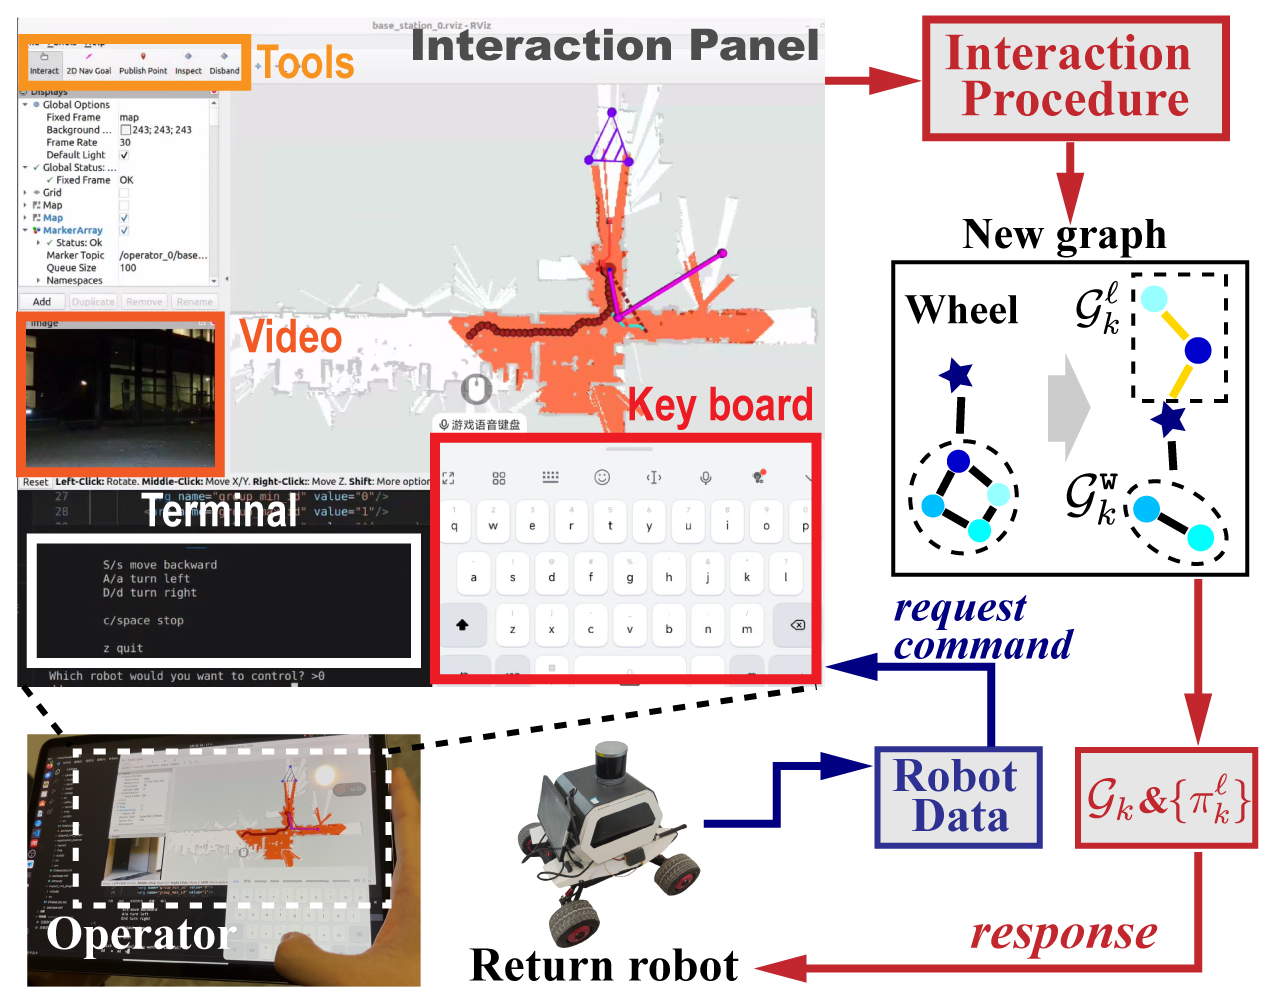
\includegraphics[width=0.95\linewidth]{figures/ch05/interaction.png}
    \vspace{-2mm}
    \caption{Illustration of the procedure on how the operator can
      interact with its team via the panels within the GUI, and the
      type of data exchanged during the return event including the
      gathered information and human commands.}
    \label{ch05:fig:interaction}
\end{figure}
%==============================

%========================================
\subsubsection{Compatibility and Sequential Request Instantiation}
\label{ch05:subsec:multi_req}
At time~$t$, the embedded graph of team~$\mathcal{T}_k$ is given by:
\begin{equation}\label{ch05:eq:decomposition}
  \mathcal{G}_k(t) \triangleq \mathcal{G}^{\texttt{w}}_k \cup
  \bigcup_{j=1}^{L_k}\mathcal{G}^{j}_k,
\end{equation}
where $\mathcal{G}^{\texttt{w}}_k$ is the wheel backbone used for
exploration, and each $\mathcal{G}^{j}_k$ is an instantiated request
subgraph that fulfills request~$\xi^{j}_k$, with $L_k$ denoting the
number of currently active requests.

Suppose robot~$\texttt{r}\in\mathcal{N}^{\texttt{w}}_k$ receives a
bundle of $L>0$ new requests
$\Xi_k\triangleq\{\xi^\ell_k\}_{\ell=1}^{L}$.
Each request~$\xi$ is associated with a candidate family of embedded
target graphs $\widehat{\mathcal{G}}_k^{\xi}$, including
\eqref{ch05:eq:frontier_weight} for $\{\xi^k_2\}$,
\eqref{ch05:eq:base-location} for $\{\xi^k_3\}$,
\eqref{ch05:eq:cec} for $\{\xi^k_4\}$ and $\{\xi^i_6\}$,
and \eqref{ch05:eq:interteam_req} for $\{\xi^{k_1k_2}_7\}$.
A subset $\Xi\subseteq\Xi_k$ is said to be \emph{compatible} on
$\mathcal{G}^{\texttt{w}}_k$ if the current wheel backbone can provide
disjoint robot subgroups for instantiating all requests in~$\Xi$, i.e.,
\begin{equation}\label{ch05:eq:compat}
  \mathcal{N}^{\xi}_k \cap \mathcal{N}^{\xi'}_k = \emptyset,\
  \forall\,\xi \neq\xi'\in\Xi;\;
  \bigcup_{\xi\in\Xi}\mathcal{N}^{\xi}_k \subseteq
  \mathcal{N}^{\texttt{w}}_k,
\end{equation}
where $\mathcal{N}^{\xi}_k$ denotes the set of robots allocated to
fulfill~$\xi$.
However, the operator-relocation request $\{\xi^k_3\}$, including both
motion within the feasible region and migration, is only compatible
with the complete wheel backbone. If the fleet is already split,
robots in detached subgraphs cannot be guaranteed to
receive the new operator location after migration. Therefore,
$\{\xi^k_3\}$ is deferred until all other active requests are completed
and the complete wheel backbone is restored.

Determining a maximum compatible subset of $\Xi_k$ under
\eqref{ch05:eq:compat} is generally combinatorial,
requiring an additional subset-selection problem at each activation event.
MoRoCo does not pursue such a globally optimal selection.
Instead, it adopts a tractable sequential policy: requests are examined according to a priority order,
and a request is retained only if it is admissible on the current wheel backbone
and $\texttt{GraphMatch}(\cdot)$ returns an executable instantiation.
The priority order is determined either by operator specification or by the default FIFO setting.
Specifically, let $\mathcal{G}^{\texttt{w},0}_k$ denote the wheel
graph before processing the new request bundle.
For $\ell=1,\cdots,L$, if request $\xi^\ell_k$ is admissible,
the remaining wheel graph $\mathcal{G}^{\texttt{w},\ell-1}_k$ is split by
instantiating a target graph from
$\widehat{\mathcal{G}}_k^{\xi^\ell_k}$ via
Alg.~\ref{ch05:alg:graphmatch}, i.e.,
%========================================
\begin{equation}\label{ch05:eq:combinatorial}
  \mathcal{G}^{\texttt{w},\ell}_k,\ {\mathcal{G}}^{\ell}_k,\
  \widehat{\pi}^{\ell}_k,\ \Pi^{\ell}_k
  \leftarrow
  \texttt{GraphMatch}\!\left(\mathcal{G}^{\texttt{w},\ell-1}_k,\,
  \widehat{\mathcal{G}}^{\ell}_k,\, \xi^{\ell}_k\right),
\end{equation}
%========================================
where $\widehat{\mathcal{G}}^{\ell}_k$ denotes the target-graph family
for $\xi^\ell_k$, ${\mathcal{G}}^{\ell}_k$ is the instantiated request
subgraph, and $\widehat{\pi}^{\ell}_k$ is the associated set of detach
tasks, consistent with \eqref{ch05:eq:single_graphmatch}.
If no executable instantiation exists for the current request on the
remaining wheel backbone, that request is deferred and the procedure
moves on to the next one in the priority order.
After all newly arrived requests have been processed, the embedded graph
$\mathcal{G}_k(t)$ in~\eqref{ch05:eq:decomposition} is augmented by the
newly instantiated subgraphs that were found executable.

%==============================
\begin{algorithm}[t]
  \caption{Overall online execution of the MoRoCo framework $\texttt{MoRoco}(\cdot)$}
  \label{ch05:alg:moroco}
  \LinesNumbered
  \SetKwInOut{Input}{Input}
  \SetKwInOut{Output}{Output}
  \Input{$\{\mathcal{G}^{\texttt{w}}_{k,0}\}$, $\{\Gamma_i\}$.}
  \Output{Local plans~$\{\Gamma_i\}$ and evolving graphs
  $\{\mathcal{G}_k\}$.}
  \While{not terminated and all teams~$\{\mathcal{T}_k\}$ in parallel}{
    \tcc{\textbf{Within the wheel graph}}
    Robot~$i\in\mathcal{N}^{\texttt{w}}_k$ executes~$\Gamma_i$ in
    parallel\;
    \uIf{meeting event $\mathbf{c}_{ij}$ occurs}{
      $\Gamma_i,\Gamma_j,\mathbf{c}^{+}_{ij}
      \leftarrow \texttt{PairCoord}(\Gamma_i,\,\Gamma_j,\,\chi_{ij})$\;
      Update embeddings of $\mathcal{G}^{\texttt{w}}_k$\;
    }

    \tcc{\textbf{Request instantiation}}
    \uIf{request bundle $\Xi_k$ received}{
      Order requests in $\Xi_k$ by priority\;
      \ForEach{request $\xi^\ell_k \in \Xi_k$}{
        \uIf{$\xi^\ell_k$ admissible on $\mathcal{G}^{\texttt{w}}_k$}{
          $\widetilde{\mathcal{G}}^{\texttt{w}}_k,\,
          \widetilde{\mathcal{G}}^\ell_k,\,
          \widetilde{\pi}^\ell_k,\,
          \widetilde{\Pi}^\ell_k
          \leftarrow
          \texttt{GraphMatch}(\mathcal{G}^{\texttt{w}}_k,\,
          \widehat{\mathcal{G}}^\ell_k,\,\xi^\ell_k)$\;
          \uIf{an executable instantiation}{
            $\mathcal{G}^{\texttt{w}}_k \leftarrow \widetilde{\mathcal{G}}^{\texttt{w}}_k$, add $\widetilde{\mathcal{G}}^\ell_k$ to $\mathcal{G}_k$\;
            Store $\widetilde{\pi}^\ell_k$ for detachment\;
          }
        }
      }
      Follow detach schedules and update~$\mathcal{G}_k$\;
    }

    \tcc{\textbf{Request execution}}
    \ForEach{active request~$\xi^\ell_k$ in parallel}{
      All robots in~$\mathcal{N}^\ell_k$ perform request~$\xi^\ell_k$\;
      \uIf{request $\xi^\ell_k$ is fulfilled}{
        Trigger rejoin procedure and update $\mathcal{G}_k$\;
      }
    }
  }
\end{algorithm}
%==============================

%========================================
\subsubsection{Online Interaction and Execution}
\label{ch05:subsec:interaction}
As shown in Fig.~\ref{ch05:fig:interaction}, each operator interacts with
the fleet through a graphical panel that supports the online requests
listed in Table~\ref{ch05:tab:requests}. At time~$t$, a command from
operator~$\texttt{h}_k$ is parsed into a request bundle
$\Xi_k \triangleq \{\xi_k^\ell\}$ with associated parameters and
transmitted to team~$\mathcal{T}_k$ via intermittent communication.
Execution is fully distributed and driven by local pairwise
coordination in Alg.~\ref{ch05:alg:coordination}. Each team maintains an
embedded communication graph $\mathcal{G}_k$, initialized as a
joint-wheel backbone
$\mathcal{G}_k=\mathcal{G}^{\texttt{w}}_{k,0}$ to satisfy the
intra-team latency bound $T^k_{\texttt{h}}$ specified by $\xi^k_1$,
while inter-team exchanges under $\{\xi^{k_1k_2}_7\}$ are constrained
by the bound $T_{\texttt{c}}$. During robot meetings, local embeddings
and data are updated and fused through $\texttt{PairCoord}(\cdot)$,
enabling latency-bounded information propagation without centralized
synchronization.

Upon receiving a new bundle $\Xi_k$, the online
coordination layer of {MoRoCo} processes the requests sequentially
under the admissibility condition~\eqref{ch05:eq:compat}, and instantiates
executable request subgraphs within the overall runtime summarized in
Alg.~\ref{ch05:alg:moroco}.
Consequently, $\mathcal{G}_k$ evolves into
the union of the wheel backbone and the subgraphs required by active
requests, such as a singleton for $\{\xi^{k_1k_2}_7\}$, a chain for
$\{\xi^k_4\}$ and $\{\xi^k_6\}$, and a star for $\{\xi^k_3\}$. Robots
detach to execute within the instantiated subgraphs, while the
remaining wheel backbone continues exploration and preserves
latency-bounded intermittent connectivity. After a request is
completed, the corresponding subgraph is removed and the involved
robots rejoin the backbone, restoring $\mathcal{G}_k$ for continued
exploration and subsequent online requests.
The following theorem states the framework-level guarantee provided by
the online execution policy in
Alg.~\ref{ch05:alg:moroco}, with the proof provided in the Appendix.

\begin{theorem}
\label{ch05:thm:moroco-complete-short}
For any team $\mathcal{T}_k$ and any finite-time arrival sequence of
request bundles, suppose that whenever a request~$\xi_k^\ell$ becomes
admissible under the compatibility condition in~\eqref{ch05:eq:compat},
there exists at least one candidate
$\mathcal{G}_k^{\xi^\ell_k}\in\widehat{\mathcal{G}}_k^{\xi^\ell_k}$
such that \eqref{ch05:eq:graphmatch_trs} returns a feasible detach and rejoin
schedule for~$\mathcal{N}_k^{\xi^\ell_k}$.
Then Alg.~\ref{ch05:alg:moroco} satisfies the following properties:
\begin{enumerate}
    \item[(I)] After each request activation or completion, the
    embedded graph $\mathcal{G}_k(t)$ remains an executable decomposition
    of the form~\eqref{ch05:eq:decomposition}, consisting of a remaining wheel
    backbone and finitely many subgraphs for active requests;
    \item[(II)] Every request that becomes admissible and is instantiated by
    Alg.~\ref{ch05:alg:moroco} is fulfilled in finite time;
    \item[(III)] There exists a finite time $t_f$ such that
    $\mathcal{G}_k(t)=\mathcal{G}_k^{\texttt{w}}$ for all $t\ge t_f$,
    i.e., all request subgraphs have been removed and the complete wheel
    backbone is restored.
\end{enumerate}
\end{theorem}
